\documentclass{article}
\usepackage{hyperref}
\usepackage{array}
\newcolumntype{M}[1]{>{\centering\arraybackslash}m{#1}}
\usepackage{geometry}
\linespread{2}
\usepackage[dvipsnames]{xcolor}
\usepackage{amsmath}
\hypersetup{
    colorlinks,
    citecolor=black,
    filecolor=black,
    linkcolor=[RGB]{51,51,153},
    urlcolor=black
}
\usepackage{graphicx}
\graphicspath{ {./} }
\usepackage{xcolor}
\usepackage{listings}
\usepackage{xparse}
\usepackage[
backend=biber,
style=numeric-verb,
sorting=none,
]{biblatex}
\addbibresource{refs.bib}

\NewDocumentCommand{\codeword}{v}{%
\texttt{\textcolor{RedViolet}{#1}}%
}

\author{Xiaohan Li, Mengxian Lv, Huilin Tang, Mengyuan Zhang}
\title{\huge{A Machine Learning Approach to Abbreviation Word Sense Disambiguation}\\
\LARGE{Homework 4 Report}}
\geometry{
    a4paper,
    total={170mm,257mm},
    }

\begin{document}
    \newgeometry{top=7cm, bottom = 3cm}
    \begin{titlepage}
        \maketitle    
    \end{titlepage}
    \newgeometry{margin=3cm}
    \tableofcontents
    \newpage
    \section{Literature Review}
    Clinical text often contains a large number of abbreviations, which have different meanings and can be ambiguous. This ambiguity can lead to errors and misinterpretations, which can have serious consequences in clinical settings. In order to eliminate ambiguity and extract information from clinical narratives, several approaches have been proposed for clinical abbreviation disambiguation.

    Machine learning has a huge potential for improving clinical abbreviation disambiguation. For example, Pakhomov et al. (2005) proposed a method for abbreviation and acronym disambiguation in clinical discourse that combines dictionary lookup and machine learning.\cite{pakhomov2005abbreviation} It describes the use of several machine learning algorithms, including decision trees, naive Bayes, and support vector machines, and evaluates the method on a set of 6,000 clinical notes. The authors report an accuracy of 92.1% in identifying the correct expansion for abbreviations and acronyms.

    More recently, Joopudi et al. (2018) proposed a convolutional neural network (CNN) approach for abbreviation disambiguation in clinical text.\cite{joopudi2018convolutional} The authors trained the model on a large dataset of annotated clinical notes and achieved state-of-the-art performance on two benchmark datasets, demonstrating the potential of deep learning techniques for improving information extraction from clinical text.

    Jaber and Martinez (2022) proposed a one-fits-all classifier to disambiguate clinical abbreviations with deep contextualized representation from pre-trained language models like Bidirectional Encoder Representation from Transformers (BERT).\cite{jaber2022disambiguating} They performed a set of experiments with different pre-trained clinical BERT models to investigate fine-tuning methods for the disambiguation of clinical abbreviations. The proposed method achieved state-of-the-art performance on two benchmark datasets, suggesting that it has the potential for improving clinical text processing tasks.

    Overall, clinical abbreviation disambiguation is an important task in clinical natural language processing. While with the development of deep learning, we have much more advanced models that can apply to this task. further studies are needed to explore how to optimize these methods and improve performance. 

    \section{Data Exploration and Preprocessing}
    \subsection{Data Exploration}
    Original data contains 75 different abbreviations, and each abbreviation comes with 500 samples with pre-annotations.\\
    In order to pick an abbreviation that could yield the most meaningful result, the following steps were taken:
    \begin{enumerate}
        \item Get number of senses for each abbreviation.\\
              One abbreviation with only 1 sense is dropped.
        \item Get standard deviation of the occurrence of each sense.
        \item The results are ranked by standard deviation from low to high, and then by number of senses from high to low.
    \end{enumerate}
    The rational is to pick the abbreviation with the most even distribution of senses, and the most number of senses.
    The final abbreviation chosen is \codeword{"CVA"}, which has 2 senses and the standard deviation of the occurrence of each sense is 39.6, resulting in a relatively even distribution of the senses.
    \subsection{Data Preprocessing}
    After careful investigation of the data. The following preprocessing steps were taken:
    \begin{enumerate}
        \item For each block of sample text provided, the text block are broken down into list of sentences using \codeword{'.'} as the delimiter. Sentences are then broken down into list of words using \codeword{' '} as the delimiter.
        \item Special characters are removed from the sentences. e.g. \codeword{'(', ')'}. If a word contains special characters, it is cut into 2 words, e.g. \codeword{'metacarpophalangeal(mp)'} would be cut into \codeword{'metacarpophalangeal'} and \codeword{'mp'}.
        \item sentences that do not contain the abbreviation are removed.
        \item If a text block contains 2 or more sentences that contain the abbreviation, the text block is split into corresponding number of text blocks, each containing only 1 sentence that contains the abbreviation.
        \item De-identified date and time in different formats are unifed into \codeword{'_%#DATE#%_'}, similarly for \codeword{'_%#ZIP#%_'}.
        \item After manual inspection, all 4 digits numbers in the data set are indeed year numbers, and are unifed into \codeword{'_%#DATE#%_'}.
    \end{enumerate}
    A total number 518 samples are generated after the preprocessing steps.
    \section{Methods}
    \subsection{Feature Extraction}
    Features explored in this project is based on \textit{n-gram} where \textit{n-1} is the window size of the \textit{n-gram}. Features are generated by combining the window size and the following feature types:
    \begin{enumerate}
        \item word only e.g. \codeword{'[word1, word2...]'}.
        \item word with direction e.g. \codeword{'[l-word1, l-word2..., r-word1, r-word2...]'}.
        \item word with direction and distance to abbreviation. e.g. \codeword{'[l-n-word1, l-(n-1)-word2..., r-1-word1, r-2-word2...]'}.
    \end{enumerate}
    $n \in (2, 3, 4, 5)$ as window sized are used in this project. Resulting a total number of $4 \times 3 = 12$ types of features.
    The final feature generated is all words combined with their respective frequencies as values. The labels are senses mapped into integers.
    \subsection{Feature Set Selection}
    The generated features are fed into a random forest classifier with hyperparameter tuning by grid search to find the best combination of features.
    The results are ranked by the F1 score of the classifier. 
    \subsubsection{Feature Set Exploration}
    Random forest classifer is used to explore the impact of the feature set on the performance of the classifier.\\
    The following graphs shows the impact of the window size given the feature type:\\
    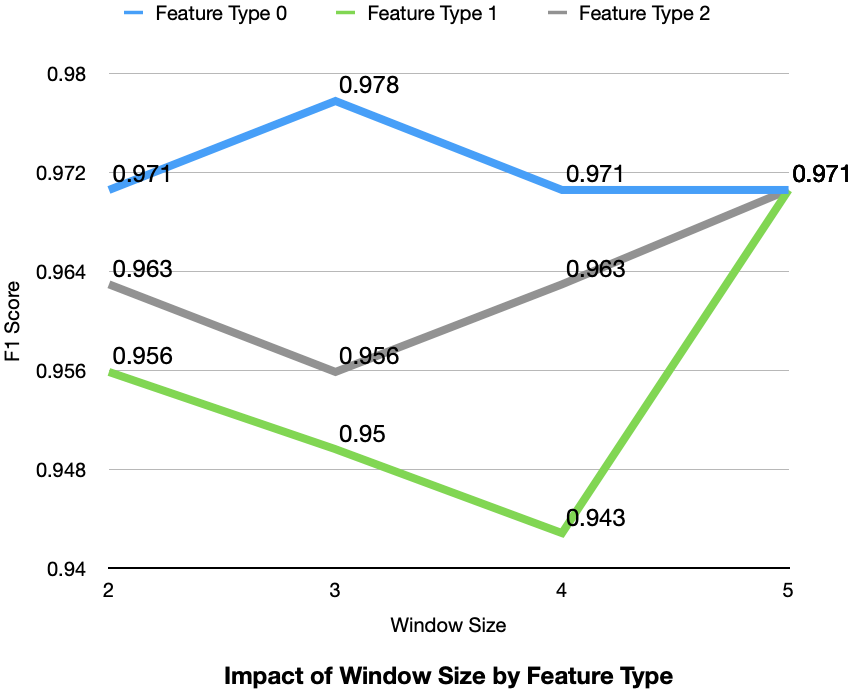
\includegraphics[width=12cm]{./by_feature.png}\\
    The following graphs shows the impact of the feature type given the window size:\\
    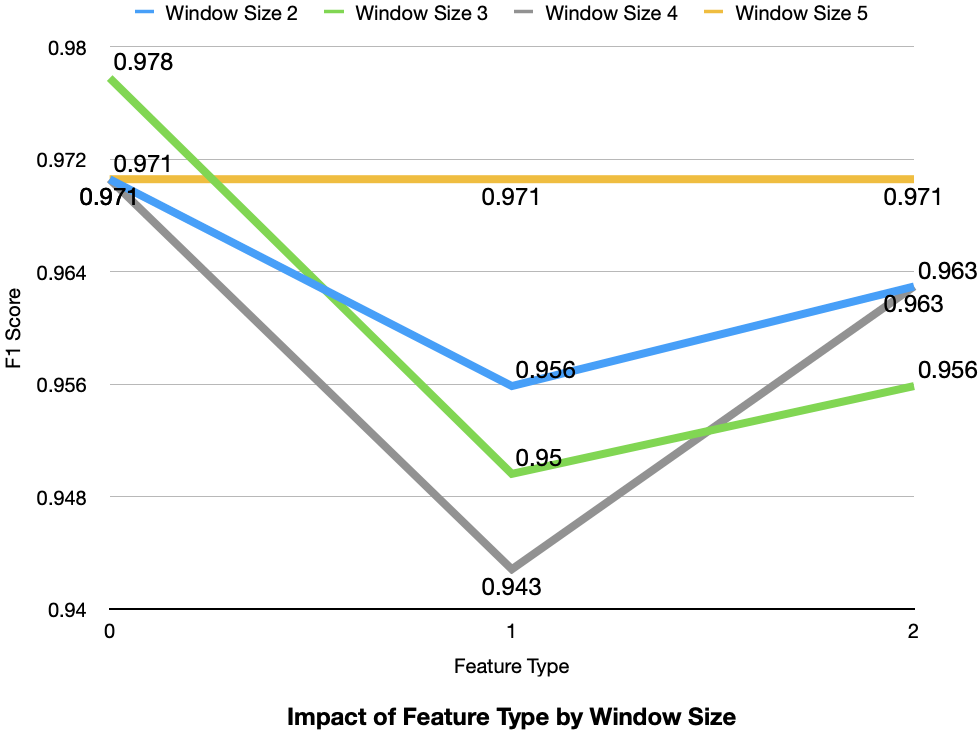
\includegraphics[width=12cm]{./by_window_size.png}\\
    \subsubsection{Best Performing Feature Set}
    The best performing set of featrues a 3-gram with basic word features, with:
    \begin{itemize}
        \item Accuracy: 99.22 (0.94\%)
        \item F1 score: 0.98
        \item ROC AUC Score:  0.97
    \end{itemize}
    \subsection{Model Selection}
    Using the best performing feature set established in the previous section, the following models are explored and compared with 5 fold stratified cross validation and grid search hyperparameter tuning (20\% out of bag data as test set):\\\\
    \begin{tabular}{|M{4cm}||M{4cm}|M{2cm}|M{2cm}|}
        \hline
        \textbf{Classifier} & \textbf{Accuracy \& STD} & \textbf{F1 Score} & \textbf{ROC AUC}\\
        \hline
        Random Forest & 99.22\% (0.88\%) & 0.98 & 0.97  \\
        \hline
        Gradient Boosting & 99.21\% (0.94\%) & 0.98 & 0.97  \\
        \hline
        Ada Boost & 97.07\% (1.99\%) & 0.98 & 0.97  \\
        \hline
        Gaussian Naive Bayes & 88.89\% (3.00\%) & 0.93 & 0.92  \\
        \hline
    \end{tabular}\\\\
    As the table suggested, random forest classifier is the best performing model with a slight edge over gradient boosting classifier.\\
    \section{Error Analysis}
    \subsection{Classification Statistics}
    Classification Report:\\\\
    \begin{tabular}{|M{3cm}||M{2.5cm}|M{2.5cm}|M{2.5cm}|M{2.5cm}|}
        \hline
            &  precision  &  recall  &f1-score  & support\\
        \hline
           0    &   0.97    &  0.95   &   0.96    &    37\\
        \hline
           1    &   0.97    &  0.99  &    0.98     &   67\\
        \hline
        accuracy     &        &       & 0.97   &    104\\
        \hline
        macro avg   &    0.97   &   0.97   &   0.97  &     104\\
        \hline
        weighted avg    &   0.97    &  0.97   &   0.97  &     104   \\
        \hline
    \end{tabular}\\\\
    The confusion matrix:\\\\
    \begin{tabular}{|M{3cm}|M{3cm}|M{3cm}|}
        \hline
        & Actual 0 & Actual 1\\
        \hline
        Predicted 0 & 35 & 2\\
        \hline
        Predicted 1 & 1 & 66\\
        \hline
    \end{tabular}\\\\
    Since the data set is somewhat imbalanced, the performance when predicting the minority class is expected to be lower than the majority class.\\
    The following table shows the data ID, actual and predicted labels of the 3 misclassified samples and the original n-gram:\\\\
    \begin{tabular}{|M{2cm}|M{2cm}|M{2cm}|M{6cm}|}
        \hline
        Data ID & Actual & Predicted & Original 3-gram\\
        \hline
        249 & 1 & 0 & ['No', 'CVA', 'tenderness']\\
        \hline
        42 & 0 & 1&['the', 'left', 'CVA', 'costal', 'margin']\\
        \hline
        69 & 0 & 1 & ['Spine', 'and', 'CVA', 'did', 'not']\\
        \hline
    \end{tabular}\\
    \subsection{Error Analysis}
    \begin{itemize}
        \item ID\_249: The sentence containing the abbreviation is only 3 word long including the abbreviation itself, and the sentence appears evenly distributed across different senses. Thus the model is unable to make a good Classification.
        \item ID\_42: After examining the data and doing some preliminary research, we found that the phrase \codeword{'CVA costal margin'} is not a commonly used combination of words since the \textit{CVA} is formed by the 12th rib and the spine while the \textit{costal margin} is an arch formed by the medical margin of the seventh rib to the tenth rib. Thus the text does not match the usual pattern of the abbreviation well enough to be classified correctly.
        \item ID\_69: The sentence containing the abbreviation is in a negative context, while 3 out of 4 words in the 3-gram are \codeword{'and'}, \codeword{'did'} and \codeword{'not'}. which are common words that are not specific to any sense. Thus the model is unable to make a good classification.
    \end{itemize}
    \section{Results and Discussions}
    In this project, almost all classifiers are able to achieve high performances. The best performing model is the random forest classifier with an accuracy of 99.22\% and F1 score of 0.98, thus is able to classify the senses of the abbreviation with high accuracy.\\
    With all window sizes except for window size 5, the performance of the machine learning algorithms exhibits a similar trend, the most basic feature set with the word only performs the best, followed by the word, direction, and position, while the word with direction features perform the worst. Looking at impact of the window size given feature type, for more complex feature sets (word, direction, with or without position), the performances tend to go down as the window size increases, but goes up significantly when the window size reaches 5, the speculation is that with more complex feature types, more data is needed to capture the patterns of the abbreviation without making the data too sparse. For the basic feature set (word only), the performance is relatively stable across all window sizes, with 3 being the local maximum, this is not expected as the window size is expected to have a positive impact on the performance, the speculation here is that most of the sentences included in the data set are short, thus often times a larger window size option is not available at all, and as the distance between the abbreviation and the context words increases, the context words become less relevant to the abbreviation, so the performance does not improve as the window size increases.\\
    Some other interesting observations are that even with manual annotations, the data set often contains false, or ambiguous, sometimes even duplicate annotations, making selecting the right, balanced abbreviation to disambiguate a key to achieving high performance in this project. \\
    However, in a more realistic scenario, the data set is often not as clean as the one used in this project, and the developer wouldn't have the luxury of hand picking the abbreviation to operate on, thus we can take a peak into what could be some of the challenges for \textit{WSD} in the real world:
    \begin{enumerate}
        \item As the number of senses increases, the need for size of the data set increases exponentially, when some senses only makes up a small portion of the data set, a traditional machine learning algorithm will likely give up on them completely, which may not be acceptable in the field of medicine sometimes.
        \item Human annotators are often not perfect, and the data set may contain false, or ambiguous, sometimes even duplicate annotations, making implementing a \textit{WSD} algorithm in the real world a labour intensive task.
        \item The meaning of a word can sometimes be related (polysemy), this may result in the words surrounding the word being somewhat similar, traditional machine learning algorithms may not be able to distinguish between the senses.
        \item Defining and understanding the context of a word is often not a trivial task.
        \item Some words could have different meaning across different domain or language, making it difficult to generalize the \textit{WSD} algorithm.
    \end{enumerate}
    In conclusion, although this project is able to achieve high performance in the \textit{WSD} task, the setting of the project is far from the real world thus making it a much easier task to achieve. To better address the challenges in the real world, methodologies beyond the scope of this project needs to be implemented.

    \newpage
    \printbibliography
\end{document}